\section{Two-Tier Probability Model}
\label{sec:sysmodel}
\begin{table}
  \center
  \caption{Notations}
  \label{tab:no}
  \begin{tabular}{c | c}
  \toprule[1pt]
    {\textbf{Notation}} & {\textbf{Explanation}} \\
  \toprule[0.5pt]
    {$\mathcal{N}$} & {the node set} \\
    {$N$} & {the number of nodes} \\
    {$i$} & {a node (station),$i \in \mathcal{N}$} \\
    {$i \rightarrow j$} & {a contact (bike trip) from $i$ to $j$} \\
    {$C^{k}_{i,j}$} & {the number of $i \rightarrow j$ in $k$th day} \\
    {$P_{i,j}^k[w]$ ($P_{i,j}^k[h]$)}
    & {inter-day prob. of $i \rightarrow j$ in weekday (weekend)} \\
    {$D_w$ ($D_h$)} & {dataset for intra-day prob. weekday (weekend)} \\
    {$\{p_{i, j}^x[w]\}$ ($\{p_{i, j}^x[h]\}$)}
    & {intra-day prob. of $i \rightarrow j$ in weekday (weekend)}\\
    {$seq_{i,j}$} & {the probability sequence of $i \rightarrow j$} \\
    {$G^{t, T}$} & {the delivery metric from time $t$ to time $T$} \\
    {$T_m$} & {the maximum message lifespan (days)}\\
  \bottomrule[1pt]
  \end{tabular}
\end{table}
In this paper, the bike station in the bike sharing system (BSS),
which can forward the message to other stations via the bike trip,
becomes the node in OppNet.
When the bike trip from node (station) $i$ to node (station) $j$ occurs,
the messages in node $i$ also can be forwarded to node $j$
through the moving bike at the same time.
Note that the message forwarding from $j$ to $i$ can not be served
by the bike trip from $i$ to $j$ simultaneously.
Thus a bike trip is a directional contact in OppNet,
which can be denoted by $i \rightarrow j$.
We assume that there exist a set of nodes $\mathcal{N}$ in OppNet
and $|\mathcal{N}| = N$.
The notations in this paper is presented in Table~\ref{tab:no}.
Since the bike trips among stations in the future are uncertain,
we design the {\it two-tier probability model} to
predict the future bike trip,
where the inter-day probability represents
whether the contact can occur on this day
and the intra-day probability means which hour the contact occurs at.
\begin{figure}
  \centering
  {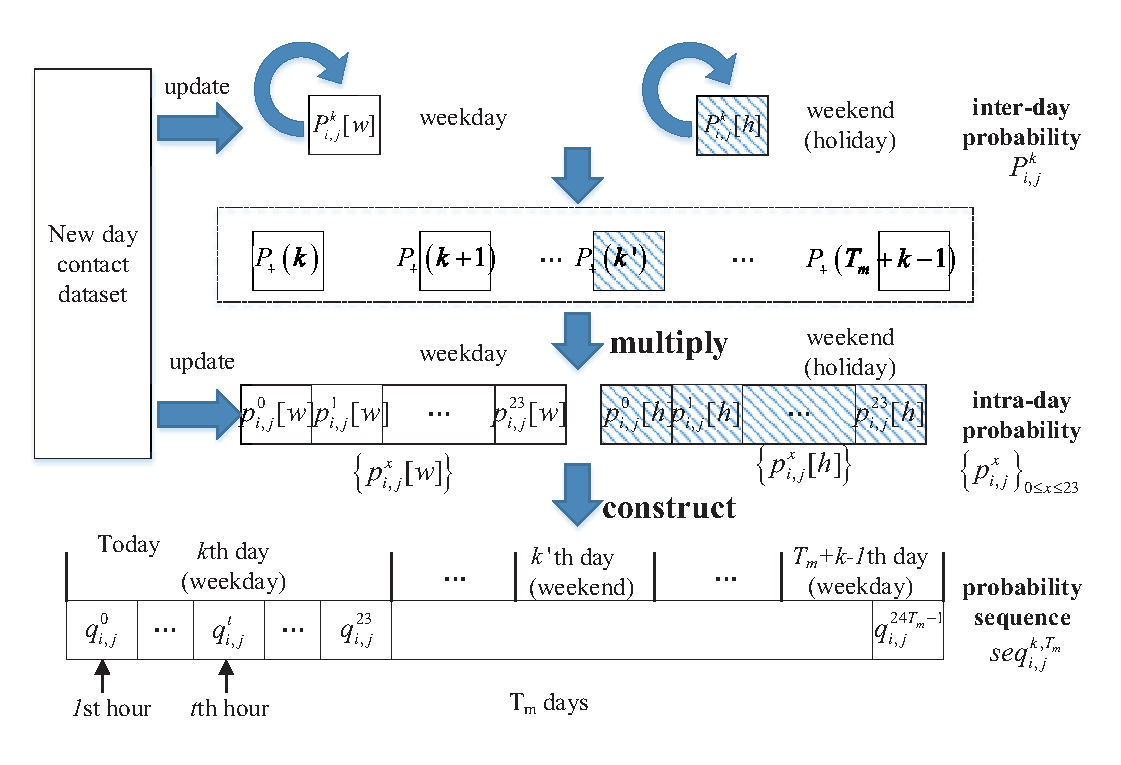
\includegraphics[width=0.47\textwidth]{fig/twotierprob.eps}}
     \caption{Two-tire probability model.}
     \label{fig:ttpm}
\end{figure}

\subsection{Inter-day probability}
\label{subsec:inter-day}
\begin{figure}
  \centering
  {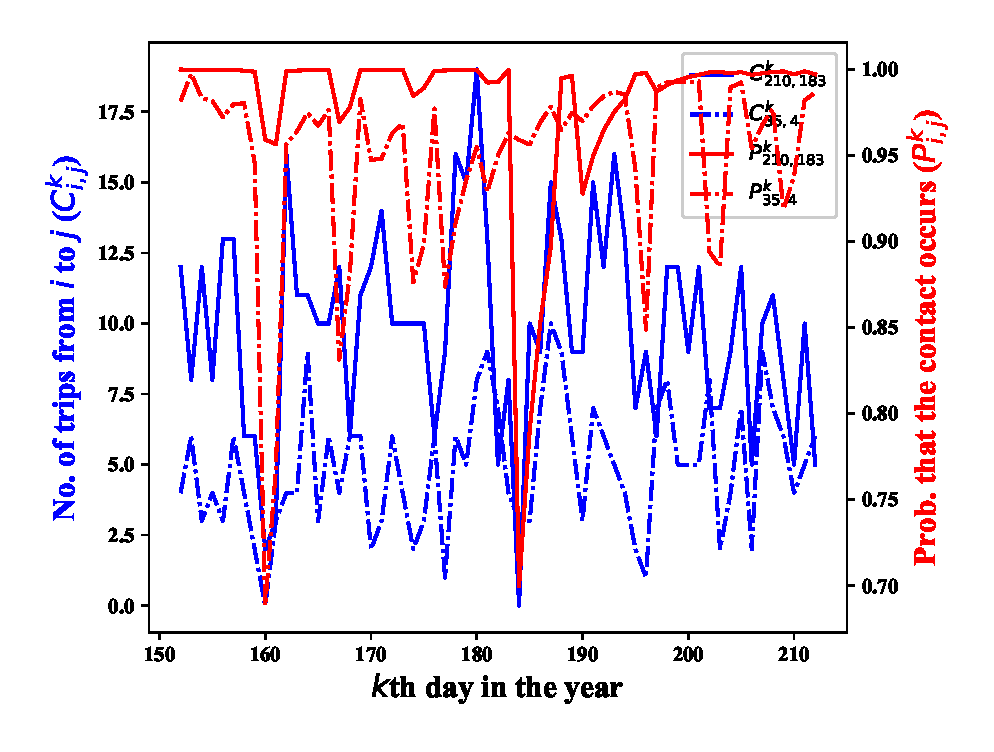
\includegraphics[width=0.47\textwidth]{fig/interdayprob_P2.eps}}
     \caption{The inter-day probability and the number of trips
     with $k$th day in a year.}
     \label{fig:interdayP}
\end{figure}
Let $C^{k}_{i,j}$ denote the number of contacts $i \rightarrow j$
in the $k$th day,
which can be collected after the end of $k$th day.
Fig.~\ref{fig:interdayP} shows that $C_{ij}^{k}$ varies
%in the two successive months, i.e., June and July, $2017$.
within around $60$ days, i.e., June and July, $2017$.
We can find that the number of contacts always changes slowly
between two successive days,
except the switch between the weekday and the weekend.
We assume that the contacts among nodes are daily periodic
and the contacts follow the Poisson process.
%Let $\bar{C}_{i,j}$ denote the expected number of contacts
%from $i$ to $j$ in the duration of one day.
Thus the probability that
at least once $i \rightarrow j$ occurs on the $k$th day,
can be estimated as
\begin{equation}
\label{eq:rho}
\begin{aligned}
\rho^{k}_{i,j} &= 1 - Prob\{\widetilde{{C}^{k}_{i,j}}=0\} \\
&= 1 - \frac{e^{-\lambda \tau}(\lambda \tau)^n}{n!} |_{\lambda \tau = {C}^{k-1}_{i,j}, n=0} \\
&= 1 - exp(-C^{k-1}_{i,j}),
\end{aligned}
\end{equation}
where $k \ge 2$.
$\widetilde{{C}^{k}_{i,j}}$ is the estimation of ${C}^{k}_{i,j}$
before the beginning of the $k$th day.
Note the estimation process of $\rho^{k}_{i,j}$ can be conducted
at least after $C^{k-1}_{i,j}$ is collected.

Since the inter-day pattern may change slowly among days caused by seasons,
%temperature, holiday/workday, weather or air pollution degree,
the inter-day probability that the contact occurs in $k$th day,
should be updated according to both $\rho^{k}_{i,j}$
and the contacts before the $k-1$th day.
Thus we use the EWMA (Exponentially Weighted Moving Average) to
predict the probability that at least once $i \rightarrow j$
occurs on the next day (e.g., the $k$th day), which is
\begin{equation}
\label{eq:P}
P^{k}_{i,j} =
\left\{
\begin{aligned}
& \rho^{k}_{i,j}, &\text{if  } k = 2 \\
& \alpha P^{k-1}_{i,j} + (1-\alpha) \rho^{k}_{i j}, &\text{if  } k \ge 3
\end{aligned}
\right.
\end{equation}
where the weight coefficient $\alpha \in (0, 1)$.
Note that at least $C^{1}_{i,j}$ should available to the prediction
and $k \ge 2$.
%$\rho_{i,j}^{k}$ can be calculated according to (\ref{eq:rho}).

The inter-day probability pattern on holidays and weekends are different
from that on weekdays, which is shown in Fig.~\ref{fig:interdayP}.
So we redefine $P^{k}_{i,j}$ as $P_{i,j}^{k}[w]$ and $P_{i,j}^{k}[h]$
for the probability estimation
on weekdays and holidays (including weekends), respectively.
Let $k$ denote the $k$th day in the range of all the weekdays
for $P_{i,j}^{k}[w]$.
And $k$ in $P_{i,j}^{k}[h]$ means the $k$th day
in the range of all the weekends,
not the $k$th day only in the chronological order.
For example, if the $k$th day is Monday,
the estimation of $P^{k}_{i,j}[h]$ depends on the last Friday
rather the last Sunday.
%Thus $\rho_{i,j}^k[h]$ and $P_{i,j}^k[h]$ are redefined as
%the estimation of the $k$th day in all the holidays.
Then the formulas of $\rho_{i,j}^k[w]$ and $P_{i,j}^k[w]$
still follow (\ref{eq:rho}) and (\ref{eq:P}), i.e.,
\begin{equation}
\label{eq:P_weekday}
P^{k}_{i,j}[w] =
\left\{
\begin{aligned}
& 1 - e^{-C^{k-1}_{i,j}},
&\text{if  } k = 2 \\
& \alpha P^{k-1}_{i,j}[w] + (1-\alpha) (1 - e^{-C^{k-1}_{i,j}}),
&\text{if  } k \ge 3
\end{aligned}
\right.
\end{equation}
where $C^{k-1}_{i,j}$ is the number of contacts on the last Friday,
i.e., the last day in the range of all the holidays.
Similarly, $P_{i,j}^{k}[h]$ can also be calculated
based on the data on the holidays.
As shown in Fig.~\ref{fig:ttpm},
the estimation of $P_{i,j}^{k}$ can track the fluctuation of $C_{i,j}^{k}$.
The switches between $P_{i,j}^{k}[w]$ and $P_{i,j}^{k}[h]$ appears
just like $C_{i,j}^{k}$ fluctuates with $k$ increasing.
We can also find that
the frequent contacts of the station pair
always can lead to the high $P_{i,j}^{k}$.
Since $210 \rightarrow 183$ occurs more frequently than $35 \rightarrow 4$,
$P_{210,183}^{k}$ is also higher than $P_{35,4}^{k}$,
which implies that $210 \rightarrow 183$ holds
the stronger direct deliveries than $35 \rightarrow 4$.
%We can calculate the probability that
%at least once $i \rightarrow j$ can occur at the beginning of each day,
%with the collected bike trips and the probability in the previous day
%for any pair of nodes.

\subsection{Intra-day probability}
\label{subsec:intra-day}
\begin{figure}
  \centering
  {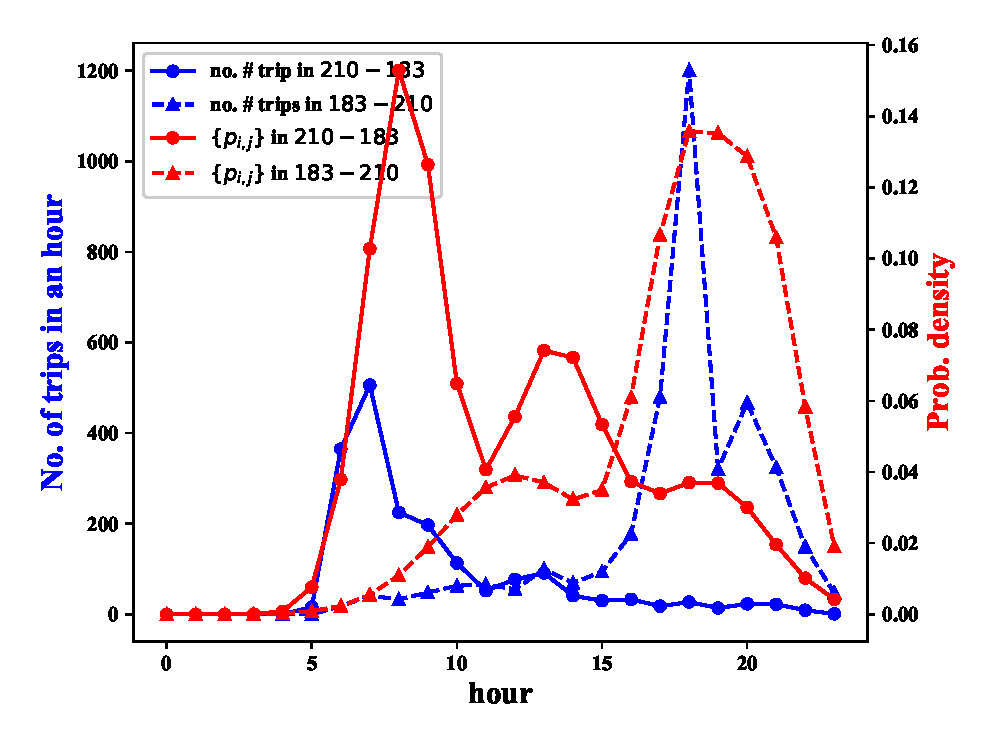
\includegraphics[width=0.47\textwidth]{fig/intradayprob_p.eps}}
     \caption{The intra-day probability density and the number of trips
     in an hour of a weekday.}
     \label{fig:intradayp}
\end{figure}
Though the intra-day probability (e.g., $P_{i,j}^k$) denotes
that there exist at least one contact in the specific day (e.g., $k$th day),
the intra-day probability density also needs to be represented.
Fig.~\ref{fig:intradayp} shows the number of bike trips changes
in different hours between node $210$ and node $183$.
We can find that there exist different pattern
between $210 \rightarrow 183$ and $183 \rightarrow 210$.
Node $210$ (node $183$) is the bike station
near the residential areas (the metro station).
The corresponding rush time of $210 \rightarrow 183$
and $183 \rightarrow 210$ is about $8:00$ and $18:00$,
which implies the commutes in the urban areas.
There also exist the different temporal distributions
in other node pairs.
%We can find that the contact probability patterns in the range of day
%are not same for any two node pair.
%The contact history from the residence to the metro station
%show the apparent peak phenomenon,
%which means that the most of contacts occur in the morning rush hour,
%i.e. $7$ a.m. to $9$ a.m..
%But the contacts from the metro station to the residence
%mainly focus in the afternoon peak hours.
%Some contacts in the rural areas will not show
%the apparent difference between the peak and the valley.
So we need to depict the intra-day probability pattern
for any node pair with the probability density function.

The gaussian mixture model (GMM), as a widespread method
of estimating the probability density function,
can be utilized to represent the probability distribution
in the range of a whole day for any $i \rightarrow j$.
For example, we want to estimate the probability density function of $i \rightarrow j$,
i.e., $p_{i j}$.
The input data of estimating GMM
is the dataset, which includes every time when $i \rightarrow j$ occurs.
Here the time can be calculated as $t_{c}.hour+t_{c}.min/60.0$,
where $t_{c}$ is the $c$th contact time of $i \rightarrow j$.
We adopt the classical Expected Maximization (EM) algorithm~\cite{EM77}
to estimate the parameters of GMM.
The details of EM algorithm will not presented in this paper.
The obtained probability density function by EM can be denoted as
\begin{equation}
\label{eq:prob_GMM}
p_{i,j}(x | \pi, \mu, \Sigma) =
\sum_{k=1}^{K} \pi_{k} \mathcal{N}(x|\mu_{k}, \Sigma_{k}).
\end{equation}
where $\mathcal{N}(x|\mu_{k}, \Sigma_{k})$ is the gaussian distribution function
with mean $\mu_{k}$ and variance $\Sigma_{k}$.
$\pi_{k}$ is the normalized weight of $\mathcal{N}(x|\mu_{k}, \Sigma_{k})$.
$p_{i,j}(x | \pi, \mu, \Sigma)$ represents the probability density function
at the time $x$,
where $x \in \mathbb{R}$ and $0 \le x < 24$.
%The domain of decimal $x$ ranges from $0$ to $24$.

To reduce the computation overhead,
we only exploit the probability density at 0:00, 1:00, $\cdots$, 23:00.
Let the array $\{p_{i,j}^x\}$ ($x \in \mathbb{N}$ and $0 \le x \le 23$)
denotes the discrete samples of
the fitted probability density (\ref{eq:prob_GMM}).
%In order to simplify the computation,
%we calculate ,
%$x \in \mathbb{N^{+}}$ and $x \le 24$, through (\ref{eq:prob_GMM}).
%$\{p_{i,j}^x\}$ is an decimal array, which consists of $24$ decimals.
%Thus $p_{i,j}^x$ is the discrete result
%of the fitted probability density function,
$p_{i,j}^x$ represents the probability that the contact occurs
in the $x+1$th hour, i.e., from x:00 to (x+1):00.
Since the pattern in weekdays is different from that in weekends,
we also should construct the intra-day weekday pattern
and the intra-day weekend pattern,
i.e., $\{p_{i, j}^{x}[w]\}$ and $\{p_{i, j}^{x}[h]\}$, respectively.
%which are maintained independently from each other.
As shown in Fig.~\ref{fig:ttpm},
$\{p_{i, j}^{x}[w]\}$ and $\{p_{i, j}^{x}[h]\}$
are maintained independently from each other.

\subsection{Probability Sequence of the Future Contacts}
\label{subsec:seq}
% Integrated Probability Sequence
Based on the proposed {\it two-tier probability model},
we can infer the probabilities of the future contacts
in the successive multiple hours,
i.e., the probability sequence.
Assume the probability sequence computation is conducted
at the beginning of today (e.g., the $k$th day).
Because the maximum lifespan of the message is $T_m$ days,
we should compute the probability sequence from
which covers the following $T_m$ days from today.
Thus the probability sequence of $i \rightarrow j$ from the $k$th day
can be denoted as
\begin{equation}
\label{eq:prob_seq}
\begin{aligned}
%seq_{i,j}^{(K-k+1) \times 24}
%seq_{i,j}
%= &(q^{k}_{0}, q^{k}_{1}, \cdots, q^{k}_{23},
%\cdots, q^{K-1}_{23}, q^{K}_{0}, \cdots, q^{K}_{23}),\\
seq_{i,j}^{k,T_m}
= &(q_{i,j}^{0}, q_{i,j}^{1}, q_{i,j}^{2}, \cdots, q_{i,j}^{24T_m -1}),\\
\end{aligned}
\end{equation}
where every $24$ successive $q_{i,j}$s correspond the probabilities on one day.
If the maximum lifespan is two days, i.e., $T_m=2$,
the probability sequence only needs to cover two days (or $48$ hours)
from $q_{i,j}^{0}$ to $q_{i,j}^{47}$.

Fig.~\ref{fig:ttpm} shows the procedure of
calculating the probability sequence for the contact $i \rightarrow j$.
The intra-day probability pattern, $P_{i,j}^{k}[w]$ and $P_{i,j}^{k}[h]$,
can be updated at the beginning of $k$th day (weekday or holiday)
based on EWMA and the collected contacts.
Meanwhile, the intra-day probability pattern,
$\{p_{i,j}^x[w]\}$ and $\{p_{i,j}^x[h]\}$,
are also updated via EM algorithm.
If the message is transmitted on the $k^{\prime}$th day eventually,
the potential contact before $k^{\prime}$th day will not occur.
Thus the probability that
the first contact occurs at $k^{\prime}$th day can be computed as
\begin{equation}
\label{eq:P_Cond}
\nonumber
\begin{aligned}
P_{+}(k^{\prime})
=& Prob\{\text{$1$st contact on $k^{\prime}$th day}\} \\
=& P^{k^{\prime}}_{i,j}\prod_{\kappa=k}^{k^{\prime}-1} (1-P^{\kappa}_{i,j}),
\end{aligned}
\end{equation}
where $P^{\kappa}_{i,j} = P^{k}_{i,j}[w]$
if the $\kappa$th day is a weekday.
Otherwise, $P^{\kappa}_{ij} = P^{k}_{i,j}[h]$.
So we need to query and record
whether the $k^{\prime}$th day ($k \le k^{\prime} \le T_m + k -1$) is a weekday
from the Internet.
Each element in the probability sequence of $i \rightarrow j$
can be calculated as
\begin{equation}
\begin{aligned}
q^{24(k^{\prime}-k)+t}_{i,j} = & Prob\{\text{$1$st contact on the $k^{\prime}$th day}\} \\
&\times Prob\{\text{the contact occurs in $t+1$th hour}\} \\
= & P_{+}(k^{\prime}) p_{i,j}^t,\\
= & P^{k^{\prime}}_{i,j}\prod_{\kappa=k}^{k^{\prime}-1}
(1-P^{\kappa}_{i,j}) p_{i,j}^t
\end{aligned}
\end{equation}
where $q^{24(k^{\prime}-k)+t}_{i,j}$ denotes the probability
that the first $i \rightarrow j$ occurs
during the $t+1$th hour of the $k^{\prime}$th day.
%$P^{k}_{i,j}$ and $p^t_{i,j}$ can be obtained from
%(\ref{eq:P_Cond}) and (\ref{eq:prob_GMM}), respectively.
Here the subscript notation $i \rightarrow j$ is eliminated
in $P_{+}(k)$ for simplifying.

The time slice in this paper is set as one hour for
balancing the computation overhead and the computation accuracy.
The probability sequence (\ref{eq:prob_seq}),
of which the element denotes the probability
that the first contact occurs in a specific hour,
is actually the discrete probability density with the granularity of one hour.
%The probability sequence of $i \rightarrow j$,
%which covers from $k$th day to $K$th day,
%is denoted by
%$(q^{k}_{1}, q^{k}_{2}, \cdots, q^{k}_{24}, q^{k+1}_{1},
%\cdots, q^{K}_{24})$.
%Here $q^{k+1}_{9}$ denotes the probability that
%a contact can occur from $i$ to $j$ between $8$ $a.m.$ and $9$ $a.m.$
%of the $k+1$th day.
%$k$ denotes $k$th day (the current day).
%$K$ denotes the $K$th day, when the lifespan of the latest message exhausts.
%At the beginning of every day,
%the probability sequences for any pair of nodes should be updated for the routing metric calculation.
%
%Without loss of generality,
%we assume the latest message,
%which is generated in $k$th day,
%will exhaust the corresponding lifespan in $K$th day.

